\section{Proposed Architecture}\label{sec:architecture}

\Cref{fig:architecture} shows the proposed architecture. White components exist in Karmada and are used without modification. Shaded components are proposed in this paper. They are not implemented yet; the implementation is part of the planned experimental study.

\begin{figure}[t]
\centering
\IfFileExists{figures/architecture.png}%
  {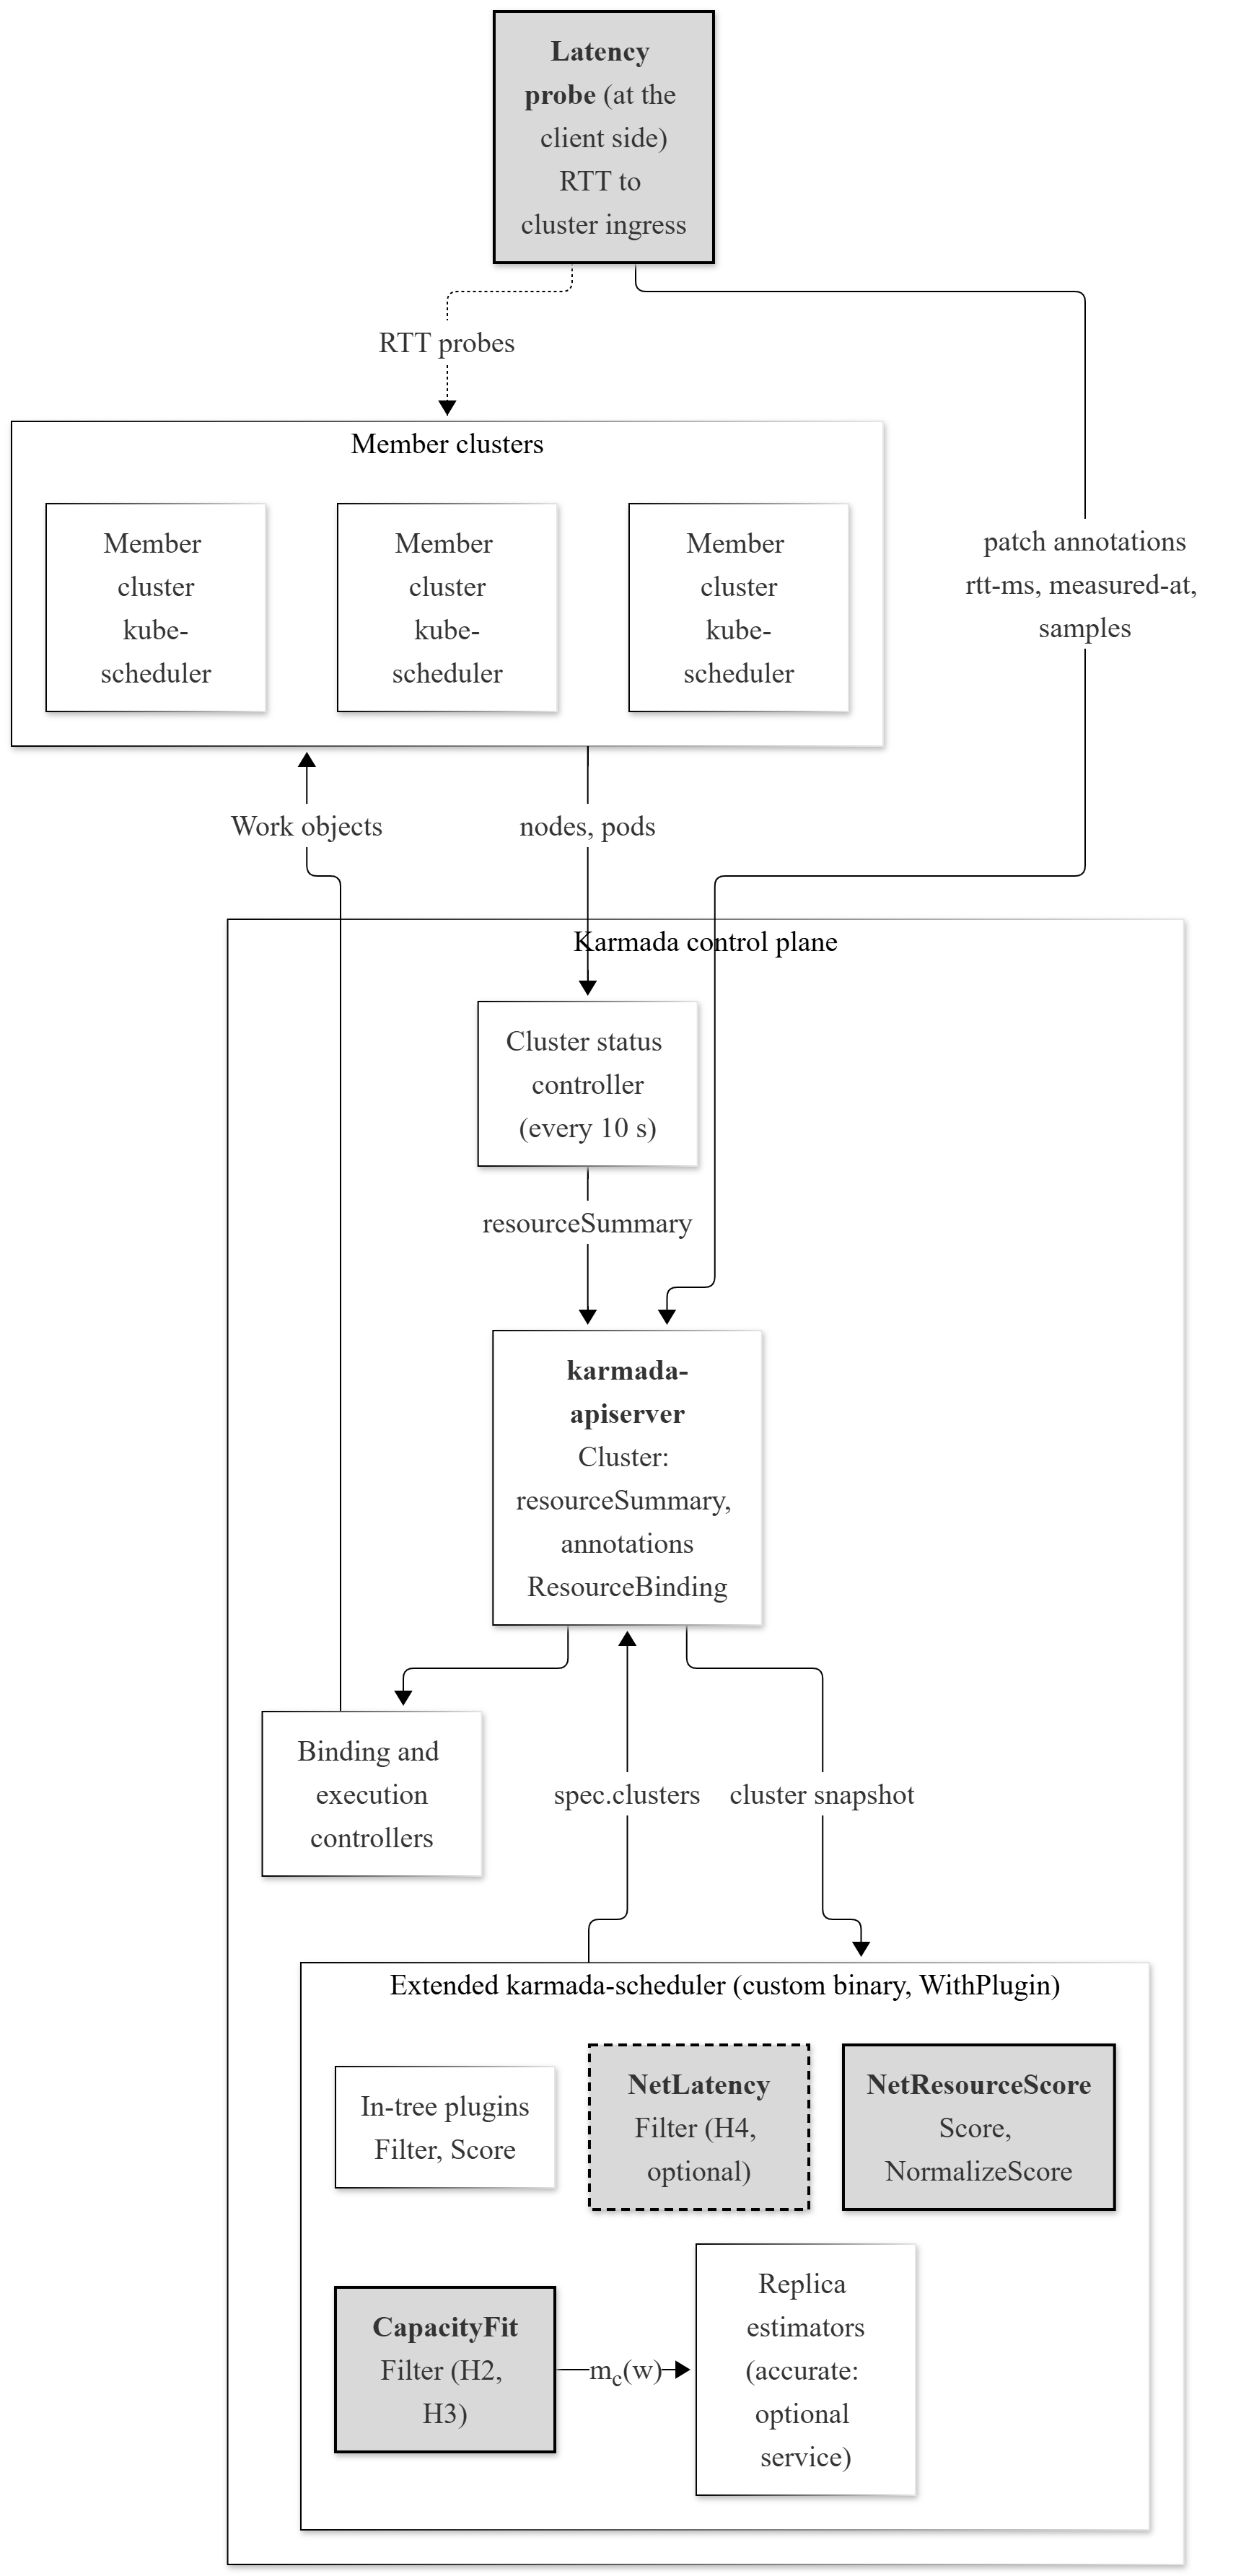
\includegraphics[width=\textwidth,height=0.7\textheight,keepaspectratio]{figures/architecture.png}}% exported from figures/mermaid/architecture.mmd
  {\resizebox{\textwidth}{!}{% Fig. 2 -- Proposed architecture. Shaded boxes = proposed components; white boxes = existing Karmada components.
\begin{tikzpicture}[
  font=\footnotesize, >={Stealth[length=2mm]},
  box/.style={draw, rounded corners=2pt, align=center, minimum height=0.8cm, inner sep=3pt},
  prop/.style={box, fill=gray!25, thick},
  exist/.style={box, fill=white},
  grp/.style={draw, rounded corners=4pt, dashed, inner sep=6pt},
  lbl/.style={font=\scriptsize\itshape, align=center}
]
% ---------------- control plane ----------------
\node[exist, minimum width=4.6cm] (api) at (0,0) {karmada-apiserver\\ \scriptsize Cluster (status.resourceSummary, annotations),\\ \scriptsize ResourceBinding};
\node[exist, minimum width=3.4cm] (ctrl) at (-5.6,0) {Cluster status controller\\ \scriptsize (every 10 s)};
\node[exist, minimum width=3.0cm] (est) at (5.4,-2.3) {Replica estimators\\ \scriptsize general / resource model /\\ \scriptsize accurate (optional)};

% extended scheduler
\node[exist, minimum width=2.6cm] (intree) at (-2.2,-2.3) {In-tree plugins\\ \scriptsize Filter, Score};
\node[prop, minimum width=2.2cm] (cap) at (0.55,-2.3) {CapacityFit\\ \scriptsize Filter};
\node[prop, minimum width=2.4cm] (nrs) at (2.95,-2.3) {NetResourceScore\\ \scriptsize Score, NormalizeScore};
\node[prop, dashed, minimum width=2.2cm] (lat) at (0.55,-3.45) {NetLatency\\ \scriptsize Filter (optional)};
\begin{scope}[on background layer]
  \node[grp, fit=(intree)(cap)(nrs)(lat), label={[lbl, anchor=south west]north west:extended karmada-scheduler (custom binary, WithPlugin)}] (sched) {};
\end{scope}
\begin{scope}[on background layer]
  \node[grp, densely dotted, inner sep=9pt, fit=(api)(ctrl)(sched)(est), label={[lbl, anchor=south east]north east:Karmada control plane}] (cp) {};
\end{scope}

% ---------------- probe and clients ----------------
\node[prop, minimum width=2.6cm] (probe) at (-5.6,2.3) {Latency probe\\ \scriptsize RTT to cluster ingress};
\node[exist, minimum width=2.0cm] (clients) at (-8.0,2.3) {Clients};

% ---------------- member clusters ----------------
\node[exist, minimum width=2.4cm] (m1) at (-4.0,-5.6) {Member cluster 1\\ \scriptsize kube-scheduler};
\node[exist, minimum width=2.4cm] (m2) at (0.0,-5.6) {Member cluster 2\\ \scriptsize kube-scheduler};
\node[exist, minimum width=2.4cm] (m3) at (4.0,-5.6) {Member cluster 3\\ \scriptsize kube-scheduler};

% ---------------- data flows ----------------
\draw[->] (m1.north) to[out=110,in=-90] node[lbl, pos=0.55, left] {nodes, pods} (ctrl.south);
\draw[->] (ctrl.east) -- node[lbl, above] {resourceSummary} (api.west);
\draw[->, thick] (probe.east) to[out=0,in=150] node[lbl, above, pos=0.45] {patch annotations\\ rtt-ms, measured-at, samples} (api.north west);
\draw[->, densely dashed] (probe.south) to[out=-100,in=180] node[lbl, pos=0.7, left] {RTT probes} (m1.west);
\draw[-, densely dotted] (clients.east) -- (probe.west);
\draw[->] ([xshift=-6mm]api.south) -- node[lbl, left] {snapshot} ([xshift=-6mm]api.south |- sched.north);
\draw[<-] ([xshift=6mm]api.south) -- node[lbl, right] {spec.clusters} ([xshift=6mm]api.south |- sched.north);
\draw[->] (cap.north) to[out=40,in=135] node[lbl, above, pos=0.6] {$m_c(w)$} (est.north west);
\draw[->] (cp.south -| m2.north) -- node[lbl, right] {Work objects (binding and execution controllers)} (m2.north);
\draw[->] (cp.south -| m3.north) -- (m3.north);
\draw[->] ([xshift=4mm]cp.south -| m1.north) -- ([xshift=4mm]m1.north);
\end{tikzpicture}
}}% TikZ fallback
\caption{Proposed architecture; shaded boxes are proposed components, white boxes are existing Karmada components}\label{fig:architecture}
\end{figure}

\subsection{Components}\label{sec:arch-components}

The \emph{extended karmada-scheduler} is the standard Karmada scheduler built with three additional plugins through the documented out-of-tree registration (property P2) \cite{karmada_docs_custom_scheduler}. All in-tree plugins remain enabled. \emph{CapacityFit} is a filter that enforces the capacity condition by calling Karmada's replica estimators (P9). \emph{NetResourceScore} is a score plugin that combines resource headroom with network suitability; its normalisation step applies the validity rules for network measurements. \emph{NetLatency} is an optional filter for workloads that require a hard latency bound; it is disabled unless explicitly configured.

The \emph{latency probe} is an external controller placed close to the client population that a scheduler instance represents. It periodically measures the round-trip time to the service entry point of each member cluster, for example by timing a TCP connection set-up, and writes the result to annotations of the corresponding Cluster object in the Karmada control plane. The probe is not on the scheduling path: a failure of the probe changes only the validity of the stored measurements.

Monitoring systems such as Prometheus may observe the scheduler and the probe, but the decision does not query them. Querying an external service inside a score plugin would add network delay to every decision and could fail, and a failure aborts the scheduling attempt (P4).

\subsection{Telemetry contract}\label{sec:arch-telemetry}

The probe and the scheduler share the annotations listed in \cref{tab:telemetry}. Annotations are used instead of labels for a specific reason. A change of Cluster labels makes the scheduler re-enqueue the bindings whose cluster affinity can match the changed cluster, whereas a change of annotations triggers no re-enqueueing (P11). With measurements refreshed every few seconds, labels would cause continuous scheduling activity. The scheduler reads the current Cluster objects from its informer cache at the start of each decision, so annotations written by the probe are visible at the next decision without causing additional scheduling activity.

\begin{table}[t]
\caption{Cluster annotations written by the latency probe (prefix is a placeholder)}\label{tab:telemetry}
\centering\small\setstretch{1.0}
\begin{tabularx}{\textwidth}{@{}p{4.6cm}p{2.6cm}L@{}}
\toprule
\textbf{Annotation} & \textbf{Format} & \textbf{Meaning} \\
\midrule
\code{netaware.lab/rtt-ms} & decimal & $\ell_c$, median of the last $q_c$ samples, in ms \\
\code{netaware.lab/rtt-measured-at} & RFC 3339, UTC & $t_c$, time of the newest sample \\
\code{netaware.lab/rtt-samples} & integer & $q_c$, number of samples behind $\ell_c$ \\
\code{netaware.lab/rtt-vantage} & string & client population that the value represents \\
\bottomrule
\end{tabularx}
\end{table}

\subsection{Existing functionality and proposed extension}\label{sec:arch-existing}

\Cref{tab:existing} separates what Karmada provides from what the design adds. The extension does not modify Karmada's selection, replica assignment, propagation, rebalancing or failover mechanisms. A workload is handled by the extension only if its PropagationPolicy names the extended scheduler; all other workloads continue to use the default scheduler.

\begin{table}[t]
\caption{Existing Karmada functionality and proposed extensions}\label{tab:existing}
\centering\small\setstretch{1.0}
\begin{tabularx}{\textwidth}{@{}Lp{2.4cm}p{5.4cm}@{}}
\toprule
\textbf{Element} & \textbf{Existing} & \textbf{Role in the design} \\
\midrule
Filter/score framework, plugin registration, scheduler name & yes & used unchanged \\
Health taints and taint toleration filter & yes & mandatory condition H1 \\
Resource summary (Allocatable, Allocated, Allocating) & yes & input of resource suitability $R_c$ \\
Replica estimators & yes, in selection & also called before ranking (CapacityFit) \\
Spread constraint with \code{maxGroups}, tie-break order & yes & used unchanged \\
Client-to-cluster latency measurement & no & latency probe, annotations \\
Resource- and network-aware score with validity rules & no & NetResourceScore \\
Hard latency bound & no & NetLatency (optional) \\
Rebalancing, descheduling, failover & yes, separate & not modified \\
\bottomrule
\end{tabularx}
\end{table}
